\experiment{CPU Scheduling Algorithms}{11/10/2023}

\section{Aim}
Implement the following CPU scheduling algorithms.
a) Round Robin
b) SJF
c) FCFS
d) Priority
Using these algorithm find turnaround time and waiting time. For all the pro-
grams, arrival time for the processes should be considered and a Gantt chart
should be displayed as output. Output should be verified with atleast 5 pro-
cesses

\section{Algorithm}
\subsection{Round Robin}
\begin{enumerate}
   \item Start
   \item Read the number of processes and their arrival time and burst time.
   \item Read the time quantum.
   \item Sort the processes based on their arrival time in increasing order.
   \item Initialize the current time to 0. If the arrival time of the first process is not 0, set the current time to the arrival time of the first process.
   \item Enqueue the first process in the ready queue.
   \item While the queue is not empty, repeat the following steps:
   \begin{enumerate}
       \item Dequeue the front process from the queue.
       \item For each process in the array of processes, if the arrival time of the process is equal to the arrival time of the current process and the process is not the current process, enqueue the process.
       \item Determine the execution time of the current process based on whether its remaining time is less than or equal to the time quantum.
       \item Reduce the remaining time of the current process by the execution time.
       \item Update the current time by adding the execution time.
       \item Print the Gantt chart for the current process.
       \item For each process in the array of processes, if the arrival time of the process is greater than the previous current time and less than or equal to the current time and the process is not the current process, enqueue the process.
       \item If the remaining time of the current process is greater than 0, enqueue the current process back to the queue and update its turn-around time and waiting time accordingly.
       \item Otherwise, update the turn-around time and waiting time of the current process based on the current time and the arrival time and burst time of the process.
       \item If the queue is now empty, enqueue the next process that arrives after the current time to the queue, print "idle" in the Gantt chart, update the current time to the arrival time of the next process, and break out of the loop.
   \end{enumerate}
   \item Print the process table and the average waiting time and turnaround time.
   \item Stop
\end{enumerate}

\subsection{Shortest Job First}
\begin{enumerate}
   \item Start
   \item Sort the processes based on their burst time in ascending order.
   \item Initialize the variables completed, prev, curr, and ct to 0, -1, -1, and 0, respectively.
   \item While the number of completed processes is less than the total number of processes do the following:
   \begin{enumerate}
       \item Set curr to -1.
       \item For each process in the array of processes, if the process has arrived, has remaining time greater than 0, and either curr is -1 or the rt of the current process is less than the rt of the process pointed by curr, set curr to the index of the current process.
       \item If curr is not -1 (i.e., a process has been selected for execution), do the following:
       \begin{enumerate}
           \item If the previously executed process is not the same as the currently selected process, print the start time and the process ID of the current process in the Gantt chart.
           \item Reduce the remaining time of the current process by 1.
           \item Increment the current time by 1.
           \item If the remaining time of the current process is 0, do the following:
           \begin{enumerate}
               \item Increment the variable completed.
               \item Compute the turn-around time of the current process as the difference between the current time and the arrival time of the process.
               \item Compute the waiting time of the current process as the difference between the tat and the burst time of the process.
           \end{enumerate}
           \item Set prev to curr.
       \end{enumerate}
       \item Otherwise do the following:
       \begin{enumerate}
           \item If the previously executed process (prev) is not -1 (i.e., there was a previous process), print the start time and "IDLE" in the Gantt chart.
           \item Set prev to -1.
           \item Increment the current time by 1.
       \end{enumerate}
   \end{enumerate}
   \item Print the process table and the average waiting time and turnaround time.
   \item Stop
\end{enumerate}

\subsection{First Come First Serve}
\begin{enumerate}
   \item Start
   \item Read the number of processes and their arrival time and burst time.
   \item Sort the processes based on their arrival time in ascending order.
   \item Initialize the completion time of the first process to the arrival time of the first process.
   \item For each process in the sorted list, do the following:
   \begin{enumerate}
       \item If it is the first process, calculate its waiting time as 0, turn around time as the burst time.
       \item If it is not the first process, check if the current time is less than the arrival time of the current process. If it is, print an IDLE state in the Gantt chart until the arrival time of the current process.
       \item Print the Gantt chart representation of the current process and update the completion time to the sum of the current time and the burst time of the current process.
       \item Calculate the waiting time of the current process as the difference between its completion time and its arrival time, and the turnaround time as the sum of its waiting time and its burst time.
   \end{enumerate}
   \item Print the completion time of the last process.
   \item Print the process table and the average waiting time and turnaround time.
   \item Stop
\end{enumerate}

\subsection{Priority Scheduling}
\begin{enumerate}
   \item Start
   \item Input the number of processes and their details including arrival time, burst time, and priority.
   \item Sort the processes in ascending order based on their arrival time.
   \item Initialize the variables completed, ct, curr, and prev.
   \item While the number of completed processes is less than n, do the following:
   \begin{enumerate}
       \item Set curr to -1.
       \item Loop through all the processes to find the process with the highest priority. If no process is found, break the loop.
       \item If a process is found, update the Gantt chart by printing the current time and the process ID. If the current process is different from the previous process, update prev to curr.
       \item Decrement the remaining time of the current process by 1, increment the current time by 1, and check if the current process has completed execution.
       \item If the current process has completed execution, update its turnaround time and waiting time, increment completed by 1, and set prev to -1.
       \item If the current process has not completed execution, update prev to curr.
       \item If no process can be executed at the current time, update the Gantt chart by printing the current time and "IDLE", and increment the current time by 1.
   \end{enumerate}
   \item Print the completion time of the last process.
   \item Print the process table and the average waiting time and turnaround time.
   \item Stop
\end{enumerate}

\section{C Program }
\begin{lstlisting}[label={list:c_program:queue}]
#include <stdio.h>
#define MAX 10

struct Process {
   int pid;        // process id
   int at;         // arrival time
   int bt;         // burst time
   int p;          // priority
   int rt;         // remaining time
   int wt;         // waiting time
   int tat;        // turnaround time
} temp, processes[MAX], *ready_queue[MAX], *cp, *p;

int front = 0, rear = 0;  // ready queue
int n, q, ct = 0, et;     // no of process, quantum time, current time, execution time, current process

void sort() {
   for (int i = 0; i < n - 1; i++) {
       for (int j = 0; j < n - i - 1; j++) {
           if (processes[j].at > processes[j + 1].at) {
               temp = processes[j];
               processes[j] = processes[j + 1];
               processes[j + 1] = temp;
           }
       }
   }
}

void enqueue(struct Process *p) {
   ready_queue[rear] = p;
   rear = (rear + 1) % MAX;
}

struct Process *dequeue() {
   p = ready_queue[front];
   front = (front + 1) % MAX;
   return p;
}

void round_robin() {
   enqueue(&processes[0]);
   printf("\nGantt Chart:\n");
   if (processes[0].at != 0)
       ct = processes[0].at;

   while (front != rear) {
       cp = dequeue();
       for (int i = 0; i < n; i++) {
           if (processes[i].at == cp->at && cp->pid != processes[i].pid)
               enqueue(&processes[i]);
       }

       et = cp->rt < q ? cp->rt : q;
       cp->rt -= et;
       ct += et;
       printf("%d | P%d | ", ct - et, cp->pid);

       for (int i = 0; i < n; i++) {
           if (processes[i].at > ct - et && processes[i].at <= ct && cp != &processes[i])
               enqueue(&processes[i]);
       }

       if (cp->rt > 0) {
           enqueue(cp);
           cp->tat = ct - cp->at;
           cp->wt += ct - cp->at - cp->tat;
       } else {
           cp->tat = ct - cp->at;
           cp->wt = cp->tat - cp->bt;
       }

       if (front == rear) {
           for (int i = 0; i < n; i++) {
               if (processes[i].at > ct) {
                   enqueue(&processes[i]);
                   printf("%d | idle | ", ct);
                   ct = processes[i].at;
                   break;
               }
           }
       }
   }
   printf("%d", ct);
}

void sjf() {
   printf("\nGantt Chart:\n");
   int completed = 0, prev = -1, curr = -1, ct = 0;

   while (completed <= n - 1) {
       curr = -1;
       for (int i = 0; i < n; i++) {
           if (processes[i].at > ct)
               break;
           if (processes[i].at <= ct && processes[i].rt > 0 && (curr == -1 || processes[i].rt < processes[curr].rt))
               curr = i;
       }

       if (curr != -1) {
           if (prev != curr)
               printf("%d | P%d | ", ct, processes[curr].pid);
           processes[curr].rt--;
           ct++;
           if (processes[curr].rt == 0) {
               completed++;
               processes[curr].tat = ct - processes[curr].at;
               processes[curr].wt = processes[curr].tat - processes[curr].bt;
           }
           prev = curr;
       } else {
           if (curr != prev)
               printf("%d | IDLE | ", ct);
           prev = -1;
           ct++;
       }
   }
   printf("%d", ct);
}

void fcfs() {
   printf("\nGantt Chart:\n");
   ct = processes[0].at;
   for (int i = 0; i < n; i++) {
       if (i == 0) {
           processes[i].wt = 0;
           processes[i].tat = processes[i].bt;
           printf("%d | p%d |", ct, processes[i].pid);
           ct += processes[i].bt;
       } else {
           if (ct < processes[i].at) {
               printf("%d | IDLE |", ct);
               ct = processes[i].at;
           }
           printf(" %d | p%d |", ct, processes[i].pid);
           processes[i].wt = ct - processes[i].at;
           processes[i].tat = processes[i].wt + processes[i].bt;
           ct += processes[i].bt;
       }
   }
   printf("%d", ct);
}

void priority() {
   printf("\nGantt Chart:\n");
   int completed = 0, ct = processes[0].at, curr = -1, prev = -1;

   while (completed <= n - 1) {
       curr = -1;
       for (int i = 0; i < n; i++) {
           if (processes[i].at > ct)
               break;
           if (processes[i].at <= ct && processes[i].rt > 0 && (curr == -1 || processes[i].p < processes[curr].p))
               curr = i;
       }

       if (curr != -1) {
           if (prev != curr)
               printf("%d | P%d | ", ct, processes[curr].pid);
           processes[curr].rt--;
           ct++;
           if (processes[curr].rt == 0) {
               completed++;
               processes[curr].tat = ct - processes[curr].at;
               processes[curr].wt = processes[curr].tat - processes[curr].bt;
               prev = -1;
           } else {
               prev = curr;
           }
       } else {
           printf("%d | IDLE | ", ct);
           ct++;
       }
   }
   printf("%d", ct);
}

void display() {
   printf("\n\nProcess Table:\n");
   printf("+-----+---------------+-------------+---------------+-----------------+\n");
   printf("| PID | Arrival Time | Burst Time | Waiting Time | Turnaround Time |\n");
   printf("+-----+---------------+-------------+---------------+-----------------+\n");

   for (int i = 0; i < n; i++)
       printf("| %3d | %13d | %11d | %13d | %15d |\n", processes[i].pid, processes[i].at, processes[i].bt, processes[i].wt, processes[i].tat);

   printf("+-----+---------------+-------------+---------------+-----------------+\n");

   float avg_wt = 0, avg_tat = 0;
   for (int i = 0; i < n; i++) {
       avg_wt += processes[i].wt;
       avg_tat += processes[i].tat;
   }
   avg_wt /= n;
   avg_tat /= n;

   printf("Average waiting time: %.2f\n", avg_wt);
   printf("Average turnaround time: %.2f\n", avg_tat);
}

void input(int c) {
    printf("Enter the number of processes: ");
    scanf("%d", &n);

    if (c != 4) {
        for (int i = 0; i < n; i++) {
            printf("Enter arrival time and burst time for process %d: ", i + 1);
            scanf("%d %d", &processes[i].at, &processes[i].bt);
            processes[i].pid = i + 1;
            processes[i].rt = processes[i].bt;
        }
    } else {
        for (int i = 0; i < n; i++) {
            printf("Enter arrival time, burst time and priority for process %d: ", i + 1);
            scanf("%d %d %d", &processes[i].at, &processes[i].bt, &processes[i].p);
            processes[i].pid = i + 1;
            processes[i].rt = processes[i].bt;
        }
    }

    if (c == 1) {
        printf("Enter time quantum: ");
        scanf("%d", &q);
    }
}

int main() {
    int choice;
    printf("1. Round Robin\n2. SJF\n3. FCFS\n4. Priority\nEnter your choice: ");
    scanf("%d", &choice);

    while (choice < 1 || choice > 4) {
        printf("Invalid choice. Enter again: ");
        scanf("%d", &choice);
    }

    input(choice);
    sort();

    switch (choice) {
        case 1:
            round_robin();
            break;
        case 2:
            sjf();
            break;
        case 3:
            fcfs();
            break;
        case 4:
            priority();
            break;
    }

    display();
    return 0;
}
\end{lstlisting}

\section{Output}
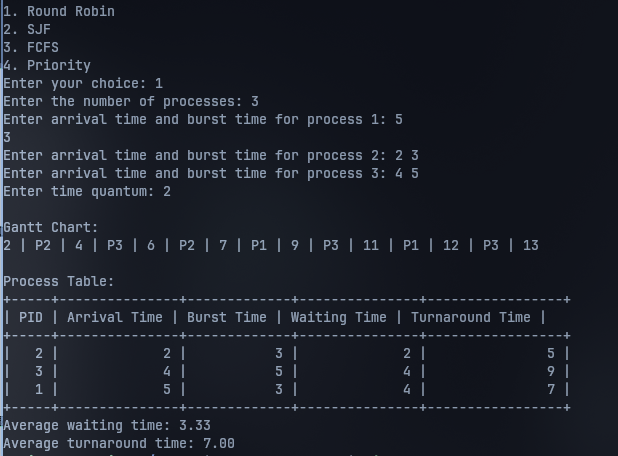
\includegraphics[\linewidth]{Cycle_2//Outputs/roundrobin.png}
\newpage
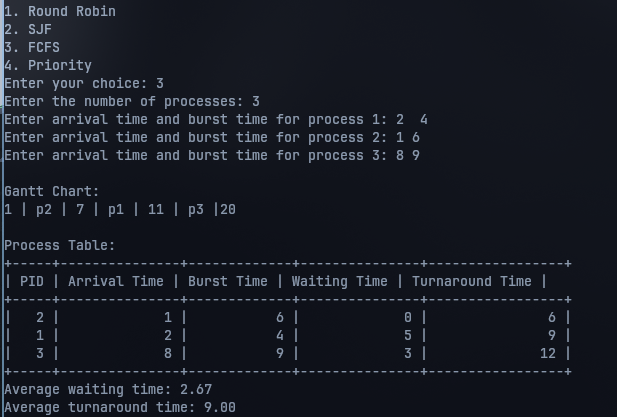
\includegraphics[\linewidth]{Cycle_2//Outputs/fcfs.png}
\newpage
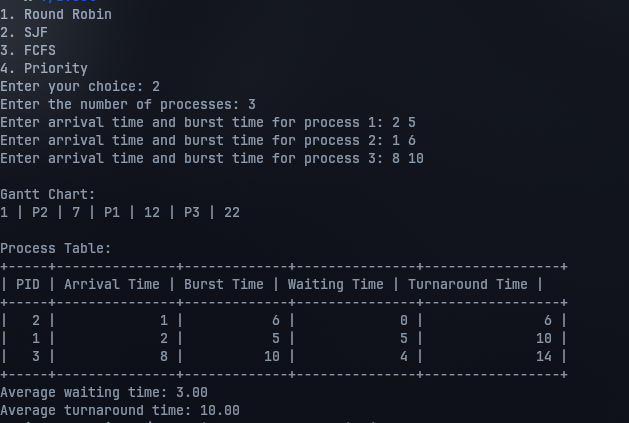
\includegraphics[]{Cycle_2/Outputs/sjf.png}
\newpage
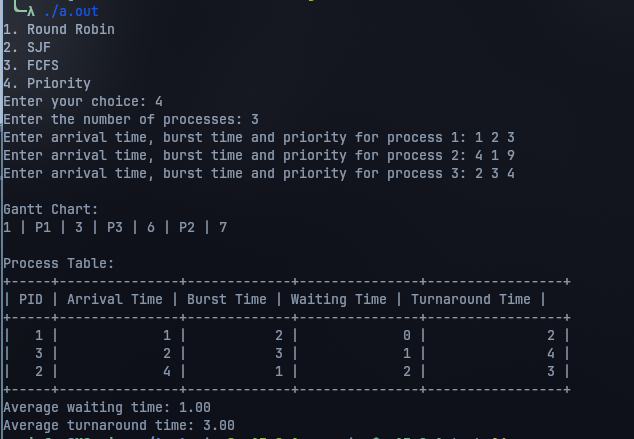
\includegraphics[]{Cycle_2//Outputs/priorityscheule.png}

\section{Result}
Executed CPU scheduling algorithms successfully